\documentclass[12pt]{article}

\usepackage{fontawesome}
\usepackage{hyperref}
\usepackage{xurl}
\usepackage{graphicx}
\usepackage{float}
\usepackage[tagged, highstructure]{accessibility}
\usepackage{bookmark}
\usepackage{enumitem}

\hypersetup{
    colorlinks=false,
    pdfborder={0 0 0},
    pdftitle={Security Video Review Lab},
    pdfauthor={Adrianna Holden-Gouveia},
    pdfsubject={Information Security - Lab Assignment},
    pdflang={en-US},
    pdfkeywords={security conferences, DEF CON, The Diana Initiative, IntroSecCon, video review, presentations}
}

% Configure PDF bookmarks for navigation
\bookmarksetup{
    numbered,
    open,
}

% Configure list spacing for better accessibility
\setlist{nosep}



\title{Security Video Review}
\author{
        Adrianna Holden-Gouveia \\
        Website: \href{https://aholdengouveia.name}{aholdengouveia.name}\\ 
        \date{\vspace{-5ex}}
        %Email: \href{mailto:admin@aholdengouveia.name}{admin@aholdengouveia.name} \\
%        \faLinkedin{: aholdengouveia} \\
        \faGithub {: aholdengouveia} \\
        \faTwitter {: aholdengouveia} \\
        }

%S\date{\today}


\begin{document}    

\maketitle

\section*{Accessibility Notice}
This document is also available in HTML format at:

Link: \href{https://aholdengouveia.name/InfoSec/labs/securityvideo.html}{\textbf{\nolinkurl{https://aholdengouveia.name/InfoSec/labs/securityvideo.html}}}

The HTML version provides enhanced accessibility features including keyboard navigation, screen reader support, responsive design, dark mode support, and high contrast options.


%\begin{abstract}
%This is a template for Linux Administration Lab work
%\end{abstract}
%\tableofcontents

\section*{Learning Outcomes}
By the end of this lab, you will be able to:
\begin{itemize}
    \item Find a security conference talk on a topic you're interested in
    \item Summarize and evaluate a talk and its presenter
    \item Compare two talks on the same topic
    \item Explain one thing you learned, and how it connects to this class
\end{itemize}

\section*{Lab Instructions}
In this lab you'll watch two talks from security conferences on the same topic, and review them. Conference talks are one of the best free ways to keep learning about security after this class.

\subsection*{Screenshots}
This lab asks for 2 screenshots, one of each talk playing. Each screenshot should have your name, term, and year.  One of the easiest ways to do that is make a text document with your name and term/year on your computer and save it to use all term. Any screenshots that don't include this information won't be counted.

\begin{figure}[H]
    \centerline{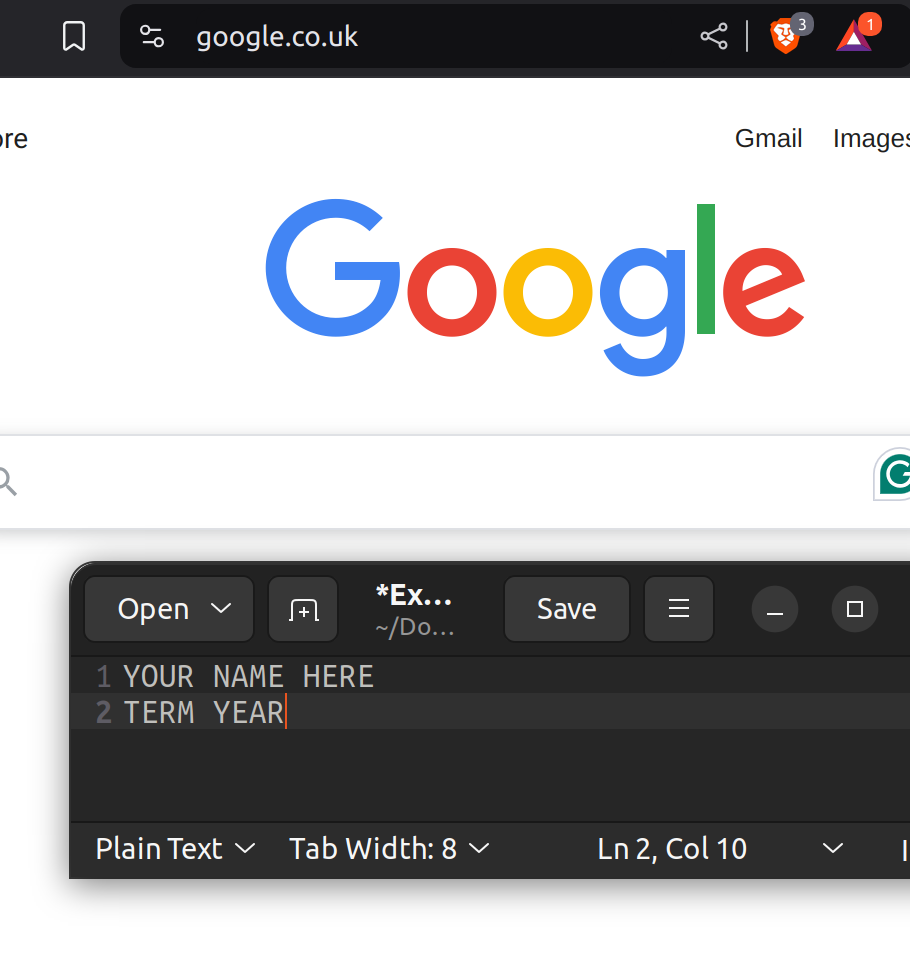
\includegraphics[scale=.2]{ExampleScreenshot.png}}
    \caption{This is an image of what each of your screenshots should look like}
    \alt{Example screenshot: a web browser showing the Google home page, with a small text editor window in front of it that says YOUR NAME HERE and TERM YEAR}
\end{figure}

\subsection*{Part 1: Pick a Talk}
Pick a talk from one of the following conferences. The talk should be from the last 2 years.
\begin{itemize}
    \item DEF CON
    Link: \href{https://www.youtube.com/@DEFCONConference/videos}{\textbf{\nolinkurl{https://www.youtube.com/@DEFCONConference/videos}}}
    \item The Diana Initiative
    Link: \href{https://www.youtube.com/@TheDianaInitiative/videos}{\textbf{\nolinkurl{https://www.youtube.com/@TheDianaInitiative/videos}}}
    \item IntroSecCon
    Link: \href{https://www.youtube.com/channel/UCx1Ektc73drCDq6W0tclZ8g}{\textbf{\nolinkurl{https://www.youtube.com/channel/UCx1Ektc73drCDq6W0tclZ8g}}} (Disclaimer: I am one of the organizers for IntroSecCon and on their board)
\end{itemize}
You can skim through the talks to find one you're interested in. If nothing interests you, you may pick a talk from another reputable security conference, but check with me first.

Take a screenshot of your talk playing, with the title showing.

\subsection*{Part 2: Review Your Talk}
Answer the following questions about the talk you picked.
\begin{enumerate}
    \item What talk did you pick? Include the title, the conference, and the link.
    \item Why did you pick it?
    \item Describe what the talk is about in a short paragraph.
    \item Who's the presenter?
    \item What's their expertise?
    \item How did they do presenting?
    \item What's one thing you thought they did well presenting? Anything they could work on?
    \item What's one thing you learned in the talk? How does it connect to something we've covered in this class?
    \item Describe one specific moment in the talk. Give the timestamp, and what was said or shown.
    \item Are you going to continue learning about this subject? Why or why not?
    \item Would you recommend this talk to others? Why or why not?
\end{enumerate}

\subsection*{Part 3: Compare a Second Talk}
Find a second talk on the same topic, by a different presenter. It can be from any of the conferences in Part 1, and should also be from the last 2 years. Take a screenshot of the second talk playing, with the title showing.
\begin{enumerate}[start=12]
    \item What second talk did you pick? Include the title, the conference, the presenter, and the link.
    \item Describe one specific moment in the second talk. Give the timestamp, and what was said or shown.
    \item What did the two talks agree on? Where did they differ?
    \item What did the second talk add that the first one didn't cover?
    \item Which presenter explained the topic more clearly, and why?
    \item If a classmate only had time for one of the two talks, which would you tell them to watch? Why?
\end{enumerate}

\section*{Deliverables}
One file that includes:
\begin{itemize}
    \item Part 1: your screenshot of your first talk playing
    \item Part 2: your answers
    \item Part 3: your screenshot of your second talk playing, and your answers
\end{itemize}

\section*{Resources}
References, a video, a PowerPoint and some notes are available at my website
Link: \href{https://www.aholdengouveia.name/InfoSec/Cryptography.html}{\textbf{\nolinkurl{https://www.aholdengouveia.name/InfoSec/Cryptography.html}}}

DEF CON talks
Link: \href{https://www.youtube.com/@DEFCONConference/videos}{\textbf{\nolinkurl{https://www.youtube.com/@DEFCONConference/videos}}}

The Diana Initiative talks
Link: \href{https://www.youtube.com/@TheDianaInitiative/videos}{\textbf{\nolinkurl{https://www.youtube.com/@TheDianaInitiative/videos}}}

IntroSecCon talks
Link: \href{https://www.youtube.com/channel/UCx1Ektc73drCDq6W0tclZ8g}{\textbf{\nolinkurl{https://www.youtube.com/channel/UCx1Ektc73drCDq6W0tclZ8g}}}

\end{document}
